\documentclass[12pt,twoside]{article}

\newcommand{\fixme}[1]{\textcolor{red}{#1}}

    \usepackage{jmlda}
    \usepackage{graphics}
    \usepackage{booktabs}
    \usepackage{wrapfig}
    \usepackage{multirow}
    \usepackage{enumitem}
    \usepackage{hyperref}
    \graphicspath{{images/}}
    % \setcounter{secnumdepth}{3}
    

    %\NOREVIEWERNOTES
    \title
        {Динамическое выравнивание многомерных временных рядов}
    \author
        {Гончаров~А.\,В., Моргачев~Г.\,И., Смирнов~В.\,, Липницкая~Т.\,} % основной список авторов, выводимый в оглавление
    \thanks{
        Работа выполнена при финансовой поддержке РФФИ, проект \No\,00-00-00000.
        Научный руководитель:  Гончаров~А.\,В.
        Задачу поставил:  Гончаров~А.\,В.
        Консультант:  Гончаров~А.\,В.
    }
    \email
        {morgachev.gi@phystech.edu, smirnov.vs@phystech.edu, tanya.lipnizky@yandex.ru}
    \organization
        {МФТИ}

    \abstract{
        В работе решается задача выбора оптимальной функции расстояния между между наборами временных рядов с общей осью времени. 
        Стандартный подход к определению расстояния между наборами основан на использовании стоимости выравнивающего пути, полученного в процессе динамического выравнивания временных осей друг относительно друга.
        \fixme{Мб не здесь?} Определенная таким образом функция расстояния будет называться \textit{функцией стоимости} выравнивания наборов рядов.
        Обобщение алгоритма выравнивания на случай наборов, состоящих более чем из одного ряда предполагает использование \textit{функции расстояния} между точками двух наборов, представляющих собой элементы пространства размерности больше единицы.
        
        В работе рассмотрены функции стоимости, полученные на основе выбора различных функций расстояния между точками наборов. Анализ полученных функций стоимости проведен на примере решения задач метрической кластеризации и метрического поиска эталонной подпоследовательности для многомерных наборов рядов.
        Работа также предлагает модификацию оптимизированного алгоритма вычисления функции стоимости выравнивания рядов, позволяющую проводить её вычисления для наборов.
        Результаты моделирования представлены на основе размеченных данных о деятельности человека полученных с носимого устройства, а также данных о движении руки в процессе написания текста, полученных с графического планшета.
        
        Обоснованность метрического подхода к решению задачи демонстрируется путем сравнения с результатами на основе авторегрессионной модели.

        \bigskip
        \textbf{Ключевые слова}: \emph {временные ряды, многомерные временные ряды, DTW}.
    }

        
    \begin{document}

    \maketitle
    \setcounter{secnumdepth}{3}
    \section{Введение}\label{intro}
        
        В целях применения алгоритмов машинного обучения для решения задач, входные данные которых представлены временными рядами, появляется необходимость определения на них функции расстояния. При этом, поточечный подход, зачастую, является малоинформативным в связи с возможными деформациями оси времени: сдвигами и растяжениями~\cite{01f4ab11a9ff49ff909094a135dcfe33}.
        Одним из способов решения этой проблемы является выравнивание временных рядов (DTW)~\cite{Keogh:1999:SUD:645803.669511} и его модификаций~\cite{journals/ida/SalvadorC07,Keogh01derivativedynamic}.
        Данный подход позволяет найти оптимальный выравнивающий путь между рядами, деформированными друг относительно друга описанными выше способами~\cite{salvador2004fastdtw}. Стоимость выравнивающего пути может быть использована в качестве расстояния между выравниваемыми объектами. \fixme{Мб не здесь?} Определенная таким образом функция расстояния будет называться \textit{функцией стоимости} выравнивания рядов.
        
        Однако, в большинстве индустриальных задач измерения в каждый имеют более одного канала. Такие данные могут быть представлены в виде \textit{наборов временных рядов} с общей осью времени, между которыми также встает вопрос об определении функции расстояния. Наборы временных рядов будет обозначаться $X = \{X^1,\dots X^l\}$, каждый $X^i \in \mathbb{R}^{n}$ \-- временной ряд длинны $n$.
        
        Модификации алгоритма выравнивания на случай подобных данных описано в \cite{Holt2007,Sanguansat2012MultipleMS}.
        В работе \cite{Holt2007} предлагается способ выравнивания наборов рядов, основанный на нормализации исходных данных и нахождении векторной нормы.
        \fixme{не надо} В \cite{Sanguansat2012MultipleMS} рассматривается алгоритм, позволяющий выполнить выравнивание временных рядов между соответственными рядами из двух наборов независимо друг от друга.
        
        \begin{figure}[h!]
            \centering
            \resizebox{0.95\textwidth}{!}{\input{images/example.pdf_tex}}
            \caption{Иллюстрация выравнивания}\label{example}
        \end{figure}
        
        В ходе классического алгоритма выравнивания рядов~\cite{??} вычисляются расстояния между точками выравниваемых рядов. \textit{Точкой набора временных рядов} в момент $t$ обозначим $X_t = \{X^1_t,\dots X^l_t\}$, где $X^i_t$ \-- измерения $i$\--го временного ряда в момент времени $t$. Таким образом, точка набора из $l$ временных рядов принадлежит пространству $\mathbb{R}^{l}$.  На рисунке~\ref{example} зеленой линией обозначена точка набора из двух временных рядов при $t=25$.
        
        Аналогично, при выравнивании наборов относительно общей временной оси, вычисляются расстояния между соответственными точками наборов. При этом получаемая функция стоимости будет зависеть от выбора функции расстояния между точками. На рисунке~\ref{example} стрелками соединены примеры сравниваемых точек, которые должны совпасть после выравнивания.

        В работе решается задача выбора оптимальной функции стоимости выравнивания наборов временных рядов с общей осью времени. Сравниваются функции расстояния между точками, порожденные $L_1$, $L_2$ нормами, а также косинусное расстояние.
        
        Для измерения качества полученных функций стоимости решаются две задачи: поиска паттернов и кластеризации, решаемые метрическими методами. Поиск паттернов происходит путем нахождения наиболее близкого участка к искомому патерну. Основой решения задачи кластеризации является метрическая иерархическая кластеризация, дающая хорошие результаты при кластеризации временных рядов~\cite{WARRENLIAO20051857,AGHABOZORGI201516}.
        
        В ходе эксперимента, предложенный подход был продемонстрирован на задачах поиска приступов эпилепсии~\cite{epi} и распознавания рукописных букв~\cite{characters} для поиска паттернов, а также измерениях акселеромента телефона в кармане человека при различной деятельности~\cite{Kwapisz:2011:ARU:1964897.1964918}.  
        
% 		% проапдейтить инфу о данных 
%         Данные \cite{Kwapisz:2011:ARU:1964897.1964918} представляют собой измерения акселерометра некоторого носимого устройства,
%         например мобильного телефона, находящегося в кармане человека, и используется для индентификации действия человека в конкретный момент времени.
%         Данные разделены на 6 классов: ходьба, бег, подъём по лестнице, спуск по лестнице, сидение, лежание.
        
        
        Кроме того, было произведено сравнению полученных результатов с результатами другого подхода к работе с временными рядами -- сравнению коэффициентов их регрессионных моделей.
        
    \section{Постановка задачи выбора функции стоимости}\label{sec:problem}
	    Изучается влияния выбора функции расстояния между точками наборов временных рядов на результат работы DTW на примере двух задач:
        \begin{enumerate}[label=\arabic*)]
            \item Поиск шаблонов в наборе временных рядов
            \item Кластеризация наборов временных рядов
        \end{enumerate} 
        Для каждой их которых введены свои метрики качества $Q_\text{поиска}, Q_\text{класт.}$,  соответственно.
	    
	    \begin{Def}{}  
	        Набором временных рядов называется множество $X = \{X^1,\dots X^l\}$, где каждый $X^i \in \mathbb{R}^{n}$ \-- временной ряд длинны $n$.
	    \end{Def}
	    \begin{Def}{}  
	        Точкой набора из $l$ временных рядов называется вектор $X_t = \{X^1_t,\dots X^l_t\} \in \mathbb{R}^l$, в котором каждой из координат соответствует значение соответствующего временного ряда в момент времени $t$.
	    \end{Def}
	    
        Имеется множество функций расстояния между $\mathfrak{R}$:
            $$\mathfrak{R} = \{\rho: \mathbb{R}^l \times \mathbb{R}^l \rightarrow \mathbb{R}_+ \}$$

        Каждой функции расстояния $\rho$ между векторами соответствует функция стоимости оптимального выравнивающего пути, получение которого описано в~\ref{sec:dtw}. Множество таких функций расстояния между наборами временных рядов из множества $\mathfrak{X}$: 
        $$\text{DTW}_{\rho}: \mathfrak{X} \times \mathfrak{X} \rightarrow \mathbb{R}_+.$$
        
        Рассматриваются следующие функций расстояния между векторами $X_t, Y_\tau$:         
        \begin{enumerate}[label=\arabic*)]
            \item $\rho_{L_1}(X_t, Y_\tau) = {\displaystyle\sum_{l = 1}^{l} |X^i_t - Y^i_\tau|}$;
            \item $\rho_{L_2}(X_t, Y_\tau) = \sqrt{\displaystyle\sum_{l = 1}^{l} (X^i_t - Y^i_\tau)^2}$;
            \item $\rho_\text{cosine}(X_t, Y_\tau) = 1 - \dfrac{(X_t, Y_\tau)}{\sqrt{(X_t, X_t)}\sqrt{(Y_\tau, Y_\tau)}}$.
        \end{enumerate}
        
        Рассматривается задача выбора оптимальной функции расстояния  между точками относительно внешних критериев качества $Q_\text{поиска}, Q_\text{класт.}$, описанных в~\ref{sec:search},~\ref{sec:clust}
        $$\rho_i^* = \argmax_\rho Q_i(\rho)$$
    
        
        Кроме того, производится сравнения качества и скорости работы данного подхода с другими используемыми методами:
        \begin{enumerate}[label=\arabic*)]
            \item Функция расстояния на основе поточечных расстояний между рядами, при равным длинах рядов:
                $$
                    ED(S_1, S_2) = \sum\limits_1^m \|s_{1i} - s_{2i}\|_2
                $$

            \item Применение авторегрессионной модели для описания ряда.
        \end{enumerate}
    
    \label{sec:dtw}\section{Алгоритм выравнивания DTW}

        В данной работе в качестве метрического расстояния между объектами предлагается использовать стоимость
        \textit{пути наименьшей стоимости} между объектами.
 
        Задано два набора временных рядов, $X, Y$ длины $n$.
        В ходе алгоритма требуется построить матрицу размера $n\times n$ c элементами $D_{ij}=\rho(X_i, Y_j)$, где $\rho$ -- выбранная функция расстояния, $X_i, Y_j$ -- точки наборов рядов.
        
        Чтобы найти наибольшее соответствие между наборами рядов нужно найти выравнивающий путь W, который минимизирует расстояние между ними.
        W - набор смежных элементов матрицы D, $w_k = (i, j)_k$.
            
            $W = w_1,w_2, ..., w_k, ..., w_K $

            $max(m_1, m_2)\leq K \leq m_1 + m_2 + 1$, где K-длина выравнивающего пути
            
        Выравнивающий путь должен удовлетворять следующим условиям:
            \begin{enumerate}[label=\arabic*)]
                \item $w_1=(1,1)$, $w_K=(n, n)$
                \item $w_k = (a, b)$, $w_{k-1}=(a', b')$ : $a-a' \leq 1$, $b-b' \leq 1$ 
                \item $w_k = (a, b)$, $w_{k-1}=(a', b')$ : $a-a' \geq 0$, $b-b'\geq 0$
            \end{enumerate}

        Оптимальный выравнивающий путь должен минимизировать выравнивающую стоимость пути:
            $$
                DTW(X, Y)=\displaystyle\sum\limits_{k=1}^{K} w_k
            $$
            
        Путь находится рекуррентно:\\
            $\gamma(i, j) = \rho(q_i, c_j) + min({\gamma(i-1, j-1), \gamma(i-1, j), \gamma(i, j-1)})$ , где $\gamma(i, j)$ суммарное расстояние, $\rho(q_i, c_j)$ расстояние в текущей клетке.
						
        Кроме того, выравнивающий путь ограничивают тем, насколько он может отклоняться от диагонали. Типичным ограничением является полоса Сако-Чиба, накладывающая условие, что путь искривления не может отклоняться от диагонали больше, чем на определённый процент клеток.
                
    \label{sec:search}\section{Задача поиска паттернов}
        
        Рассматривается задача поиска заранее известных паттернов в наборах временных рядов. 
        Имеется набор временных рядов $X$ длинны $n$, содержащий сегменты класса $\mathfrak{P}$.
        Класс $\mathfrak{P}$ \-- в нашем случае, набор временных рядов длины $m \ll n$. \\
        Известо $k$ представителей класса $\mathfrak{P}$, \textit{не содержащихся в $X$}. \\
        Необходимо найти участки $S$, соответствующие данному классу. \\
        Обозначим множество начал таких участков как $\mathfrak{T} = \{t_1, \dots, t_j \}$.

        Будем считать участок найденным, если его пересечение с предполагаемым участком более $80\%$ длины $m$.
        Поиск будет проводиться путем нахождения расстояния с помощью $DTW_{\rho}$ между фрагментами набора рядов $X$ и шаблоном, полученным из известных экземпляров класса. 

        Рассматриваемая функция качества:
        \begin{align*}
            Q_{\text{поиска}}(DTW_{\rho}) = \dfrac{\sum\limits_{i=1}^j [t_i \-- \text{найден}]}{j}.
        \end{align*}

    \label{sec:clust}\section{Задача кластеризации}
        Исходные данные представляют собой наборы временных рядов длины $n$.
        Имеется выборка $ \mathfrak{X}$ из $N$ элементов.
        Для каждого элемента выборки $X$ известна метка класса $y \in \mathfrak{Y}$, где $\mathfrak{Y}$ \-- множество меток классов.

        Определим матрицу попарных расстояния:
        $$D(\text{DTW}_\rho(\mathfrak{X})) = ||D_{ij}||, \ \ D_{ij} = \text{DTW}_\rho(X, Z),\ \ X, Z \in \mathfrak{X}.$$
        И модель кластеризации:
        $$
            f: D \rightarrow \mathfrak{S}^N
        $$

        Где $\mathfrak{S}$ \-- множество меток кластеров.
        Будем рассматривать следующие функции качества:
        \begin{align*}
            Q_{\text{поиска} 1}(f(D), \mathfrak{X}) &= \frac{1}{|S|}\sum\limits_{s \in \mathfrak{S}} \max_y \frac{N_s^y}{N_s}  \\
            Q_{\text{поиска} 2}(f(D), \mathfrak{X}) &= \frac{1}{|\mathfrak{S}|}\sum\limits_{s \in \mathfrak{S}} \max_y \frac{(N_s^y)^2}{N_s N^y}
            % Q(f(D), S) = \frac{\sum\limits_{s_i, s_j \in S} \mathbb{I}(z_i = z_j \land  y_i = y_j)}{N^2}            
        \end{align*}
        Здесь: 
        \begin{itemize}[label=$\bullet$]
            \item $N_s$ \-- количество элементов в кластере с меткой $s$. 
            \item $N^y$ \-- количество элементов в классе $y$.
            \item $N_s^y$ \-- количество элементов класса $y$ в классе $s$.
        \end{itemize}

        % Пусть $s_i \in \mathbb{R}^n $ - временные ряды, являющиеся объектами некоторой выборки,
        % $\rho$ - некоторые выбранные метрики, $Q$ - критерий качества (данные с соизмеримым количеством точек), являющийся ответом.
        % Требуется постороить такую функцию выравнивания, что:
        % $ f = argmin(Q(s_i, \rho))$
                

	\paragraph{Описание алгоритма кластеризации}      
        В качестве алгоритма кластеризации используется иерархическая кластеризация, которая базируется на последовательном слияние ближайших кластеров.
        Рассматриваются различные функции расстояния между кластерами: 
        \begin{enumerate}
            \item \textit{complete:}  $d(A, B) = \max\limits_{a \in A, b \in B}(dist(a, b))$ 
            \item \textit{weighted:}  $d(A,B) = \dfrac{(dist(S,B) + dist(T,B))}{2}$, где кластер $A = S \cup T$
            \item \textit{average:}   $d(A,B) = \sum\limits_{a \in A, b \in B} \dfrac{d(a, b)}{(|A|*|B|)}$ 
        \end{enumerate} 
                
    % TODO: formal check it
    \section{Оптимизации}
        \fixme{\Large{Раздел в разработке}}
    %     В основу нашей реализации легла работа \cite{Rakthanmanon:2012:SMT:2339530.2339576}, в которой было
    %     использовано большое количество оптимизаций, позволяющих как сократить время вычисления расстояния 
    %     между рядами, так и, при возможности, вообще не вычислять его. 
    %     В ходе работы мы постарались обобщить эти оптимизации на многомерный случай.
    %     Ниже приведено их краткое описание. 

    %     \paragraph{Использование квадрата расстояния}	
    %     В DTW вычисляется квадратный корень, однако, если упустить этот шаг,
    %     относительное расстояние не изменится, поскольку обе функции монотонны и вогнуты.
    %     Это упрощает вычисления и позволяет сделать модель легкой для понимания.
    %     Таким образом, говоря о DTW, мы подразумеваем квадратные аналоги.
        
    %     \paragraph{Использование нижней границы}
    %     Для того чтобы ускорить последовательный поиск в DTW, используется нижняя граница (Lower Bounding),
    %     чтобы отбросить неподходящие последовательности (подпоследовательности).
    %     Оптимизация ускоряет поиск ещё и потому что не требует затратных вычислений.
        
    %     В эксперименте используется каскадная нижняя граница.
    %     Вначале последовательность проходит проверку на требования $LB_{Kim}$,
    %     которая использует расстояние между максимальными значениями рядов и минимальными значениями рядов.
    %     Однако, для того чтобы сравнить последовательности, они должны быть нормализованы,
    %     поэтому значения двух расстояний между максимальными и минимальными точками могут быть ничтожно малы.
    %     В случае если последовательность удовлетворила требованиям $LB_{Kim}$, происходит вторичная проверка $LB_{Keogh}$, использующей ED.
        
    %     Также бывает полезным менять роли сравниваемых последовательностей для $LB_{Keogh}$,
    %     от этого будет меняться решение к какой последовательности применяется нижняя граница,
    %     причем результаты вычисления этих границ для каждой из последовательностей при их сравнении в общем случае не будут равны.
    %     Однако данный метод применяется опционально и только в том случае, если другие нижние границы не проявили себя.
        
    %     \paragraph{Использование верхней границы}
    %     При вычислении $LB_{Keogh}$, мы можем заметить,
    %     что текущая сумма расстояний между каждой парой точек привысила определённое (наибольшее возможное) значение,
    %     в таком случае мы можем прекратить подсчёт, тк дальнейший действия дадут ещё более высокий результат.
        
    %     Если вся $LB_{Keogh}$ была посчитана и мы обнаружили, что должны вычислить DTW полностью,
    %     есть способ отбросить лишние вычислительные затраты на стадии подсчёта DTW.
    %     Если постепенно вычислять DTW слева направо от 1 до k и суммировать частичное накопление DTW с вкладом от $LB_{Keogh}$ от k+1 до n.
    %     Сумма $DTW(S_{1:k}^i, S_{1:k}^j) + LB_{Keogh}(S_{k+1:n}^i, S_{k+1:n}^j)$ является нижней границей для $DTW(S_{1:n}^i, S_{1:n}^j)$.
    %     Если в какой-то момент такая нижняя граница превысит верхнюю, расчёт прекращается.
    %     Кроме того, расходы на расчёт такой границы незначительны.
        
    %     % Мы не переделали программу для ED, напишу на питоне

    %     % Практически очевидно, что для сравнения двух временных рядов они должны быть нормализованы.
    %     % Однако она занимает больше времени, чем подсчёт ED. Таким образом было решено объединить ED ($LB_Keogh$) c Z-нормализацией.
    %     % Постепенно вычисляя нормализацию, мы в той же точке вычисляем ED ($LB_{Keogh}$).
    %     % Это позволяет отбросить неподходящую последовательность не только на стадии подсчёта дистанции, но и на стадии нормализации.
        
    %     Во многих случаях становится полезным изменить порядок поиска верхней границы.
    %     Очевидно, что разный порядок поиска приносит разное ускорение, более того существует n! выриантов упорядочивания.
    %     Чтобы найти оптимальный вариант, предлагается отсортировать индексы основанных на абсолютных значениях Z-нормализованной последовательности.
    %     Одно значение временного ряда $S_i$ сравнивается со многими из ряда $S_j$, которые далее сортируются по убыванию вклада ED. 
    %     % Такая сортировка может быть применена как к $LB_{Keogh}$, так и к отбрасыванию неподходящей последовательности на стадии нормализации.
		
		
		
		
						
    \section{Эксперимент}

        \paragraph{Нахождение подпоследовательностей}
        Использовалось две выборки, первая из которых состояла из временных рядов длиной в 182 точки с тремя каналами, соответсвующих координатам $X, Y$ 
            и силе нажатия на экран планшета.
        Вторая выборка состояла из временных рядов активности мозга в разных состояниях: эпилепсия, ходьба, бег, просмотр картинок и имеет длину элемента в 206 точек.
        Второй датасет имел многократно меньший размер, но при этом он значительно отличается от первого: периоды повторения паттернов значительно меньше.

        В обеих выборках из каждого класса выбиралось случайное подмножество представителей, из которых,
            путем усреднения методами $DBA$ и простым средним, получались поисковые шаблоны. 
        Путем склейки оставшихся рядов в случайном порядке, создавался длинный ряд, в котором производился поиск $k$ наиболее близких фрагментов 
            для каждого из шаблонов с использованием $ED$ и $DTW_\rho$ с различными $\rho$ в качестве функций расстояния.
            
        Для оценки погрешностей измерений, описанная процедура была проведена с большим количество (20) выборок, полученными из исходной с помощью бутстрепа.    
    
        \begin{table}[h]
            \centering
            \begin{tabular}{c|c *{2}{|*{3}{c}}}  
                \toprule
                  \multirow{2}{*}{$\rho$}& \multirow{2}{*}{average} & 
                            \multicolumn{3}{c|}{characters} & \multicolumn{3}{c}{epi} \\
                \cmidrule(r){3-8}
                                   &  & $Q$ & $t$ & $t_{\text{no optim}}$ & $Q$ & $t$ & $t_{\text{no optim}}$ \\
                \midrule
            \multirow{2}{*}{$L_1$} 
                    & DBA    & $0.83\pm 0.14$ & $2.85\pm 0.43$ & $11\pm 1$ & $0.53\pm 0.10$ & $26\pm 1$ & $25\pm 1$ \\
                    & mean   & $0.87\pm 0.12$ & $2.77\pm 0.45$ & $14\pm 1$ & $0.49\pm 0.08$ & $26\pm 1$ & $28\pm 2$\\
                    
            \midrule\multirow{2}{*}{$L_2$} 
                    & DBA    & $0.80\pm 0.17$ & $2.24\pm 0.30$ & $13\pm 1$ & $0.55\pm 0.07$ & $23\pm 1$ & $26\pm 2$ \\
                    & mean   & $0.84\pm 0.13$ & $2.17\pm 0.22$ & $10\pm 1$ & $0.48\pm 0.10$ & $23\pm 1$ & $26\pm 2$ \\
                    
            \midrule\multirow{2}{*}{$\text{cosine\_dist}$} 
                    & DBA    & $0.77\pm 0.18$ & $3.42\pm 1.00$ & $16\pm 1$ & $0.35\pm 0.10$ & $29\pm 2$ & $38\pm 2$ \\
                    & mean   & $0.81\pm 0.15$ & $3.43\pm 0.83$ & $14\pm 1$ & $0.27\pm 0.06$ & $26\pm 2$ & $38\pm 1$ \\
            \midrule     
            \multirow{2}{*}{ED}
                    & DBA    &   0.08   &   17.511   &    17.511   &    0.172  &   1.620   &    1.620   \\
                    & mean   &   0.09   &   17.645   &    17.645   &    0.172  &   1.540   &    1.540    \\
            \bottomrule
            \end{tabular}
            \caption{Поиск паттернов.}
        \end{table}

        Можно заметить, что на всех данных использование $L_1$ метрики дало лучшие результаты в данной задаче.
        При этом оптимизации позволили сократить время работы в более чем 5 раз на большом датасете (цифры),
            но незначительно в малом, при этом сохранив результаты.

        
        \paragraph{Кластеризация}
        В ходе эксперимента были использованы данные акселерометра мобильного телефона.
        Они представляли собой временные ряды длинной в 600 точек ускорений по осям $X, Y, Z$.
        Из них методом бутстрепа были сгенерированы 20 выборок из 600 рядов по 50 точек в каждом. 
        Каждых из рядов принадлежал к одному из четырёх возможных классов. Данные были равномерно распределены по всем классам.

        Для $DTW$, $ED$ вычислялись матрицы попарных расстояний между парами рядов, на основе которых проводилась кластеризация описанными выше методами.
        В качестве функий расстояния между векторами использовались метрики, порождённые $L_1$  и $L_2$ нормами.
        Кроме того, для каждого из временных рядов была обучена авторегрессионная модель, на основе коэффициентов которых также произведена кластеризация.
        Так как в процессе получения данных были возможны различные положения телефона в кармане, кластеризация проводилась на 4, 12, 24, 36 и 48 кластеров.

        \begin{table}[h]
            \centering
            \begin{tabular}{c|c *{2}{|*{3}{c}}}
                \toprule
                \multirow{2}{*}{$\rho$} & \multirow{2}{*}{$N_{clust}$} & \multicolumn{3}{c|}{$Q_1$} & \multicolumn{3}{c}{$Q_2$} \\
                \cmidrule(r){3-8}
                && \textit{complete} & \textit{average} & \textit{weighted} & \textit{complete} & \textit{average} & \textit{weighted} \\
                \midrule
            \multirow{5}{*}{$L_1$}
                    &  4 & $0.42\pm 0.07$ & $0.51\pm 0.07$ & $0.55\pm 0.06$ & $0.22\pm 0.09$ & $0.31\pm 0.10$ & $0.36\pm 0.09$ \\
                    & 12 & $0.46\pm 0.09$ & $0.54\pm 0.04$ & $0.57\pm 0.04$ & $0.24\pm 0.05$ & $0.33\pm 0.05$ & $0.36\pm 0.05$ \\
                    & 24 & $0.50\pm 0.03$ & $0.57\pm 0.03$ & $0.59\pm 0.03$ & $0.28\pm 0.03$ & $0.36\pm 0.04$ & $0.38\pm 0.04$ \\
                    & 36 & $0.55\pm 0.02$ & $0.60\pm 0.02$ & $0.61\pm 0.03$ & $0.33\pm 0.03$ & $0.40\pm 0.03$ & $0.41\pm 0.05$ \\
                    & 48 & $0.58\pm 0.02$ & $0.63\pm 0.02$ & $0.64\pm 0.03$ & $0.37\pm 0.03$ & $0.43\pm 0.03$ & $0.44\pm 0.04$ \\
            \midrule
            \multirow{5}{*}{$L_2$}
                    &  4 & $0.42\pm 0.06$ & $0.47\pm 0.07$ & $0.54\pm 0.06$ & $0.22\pm 0.07$ & $0.26\pm 0.09$ & $0.35\pm 0.09$\\
                    & 12 & $0.46\pm 0.04$ & $0.53\pm 0.04$ & $0.59\pm 0.04$ & $0.25\pm 0.05$ & $0.32\pm 0.05$ & $0.39\pm 0.05$ \\
                    & 24 & $0.50\pm 0.03$ & $0.57\pm 0.03$ & $0.59\pm 0.03$ & $0.28\pm 0.03$ & $0.35\pm 0.04$ & $0.39\pm 0.03$ \\
                    & 36 & $0.54\pm 0.03$ & $0.60\pm 0.03$ & $0.62\pm 0.03$ & $0.33\pm 0.03$ & $0.40\pm 0.04$ & $0.42\pm 0.03$ \\
                    & 48 & $0.58\pm 0.02$ & $0.63\pm 0.03$ & $0.64\pm 0.03$ & $0.37\pm 0.03$ & $0.43\pm 0.04$ & $0.46\pm 0.04$ \\
            \midrule
            \multirow{5}{*}{$AR$}
                    &  4 & \multicolumn{3}{c|}{$0.52\pm 0.06$} & \multicolumn{3}{c|}{$0.32\pm 0.08$}\\
                    & 12 & \multicolumn{3}{c|}{$0.61\pm 0.05$} & \multicolumn{3}{c|}{$0.42\pm 0.06$} \\
                    & 24 & \multicolumn{3}{c|}{$0.67\pm 0.05$} & \multicolumn{3}{c|}{$0.51\pm 0.07$} \\
                    & 36 & \multicolumn{3}{c|}{$0.70\pm 0.03$} & \multicolumn{3}{c|}{$0.55\pm 0.05$} \\
                    & 48 & \multicolumn{3}{c|}{$0.73\pm 0.03$} & \multicolumn{3}{c|}{$0.59\pm 0.05$} \\
            \bottomrule
            \end{tabular}
            \caption{Кластеризация.}
        \end{table}

    В большинстве случаев лучшие результаты показал метод кластеризации $weighted$.
    При этом, методы выравнивания с $L_1$ и $L_2$ метриками показали примерно равные результаты. Простейшая регрессионная модель позволила достичь лучшего качества во всех экспериментах.
						
    На картинках \ref{img1}, \ref{img2} приводится примеры рядов, отнесенных к одному кластеру,
        выравненных относительно случайного набора рядов из данного кластера для $L_1$ и $L_2$ метрик соответственно.
    Кластеризация в данных примерах проводилась с помощью метода $weighted$.

    \begin{figure}[h!]
        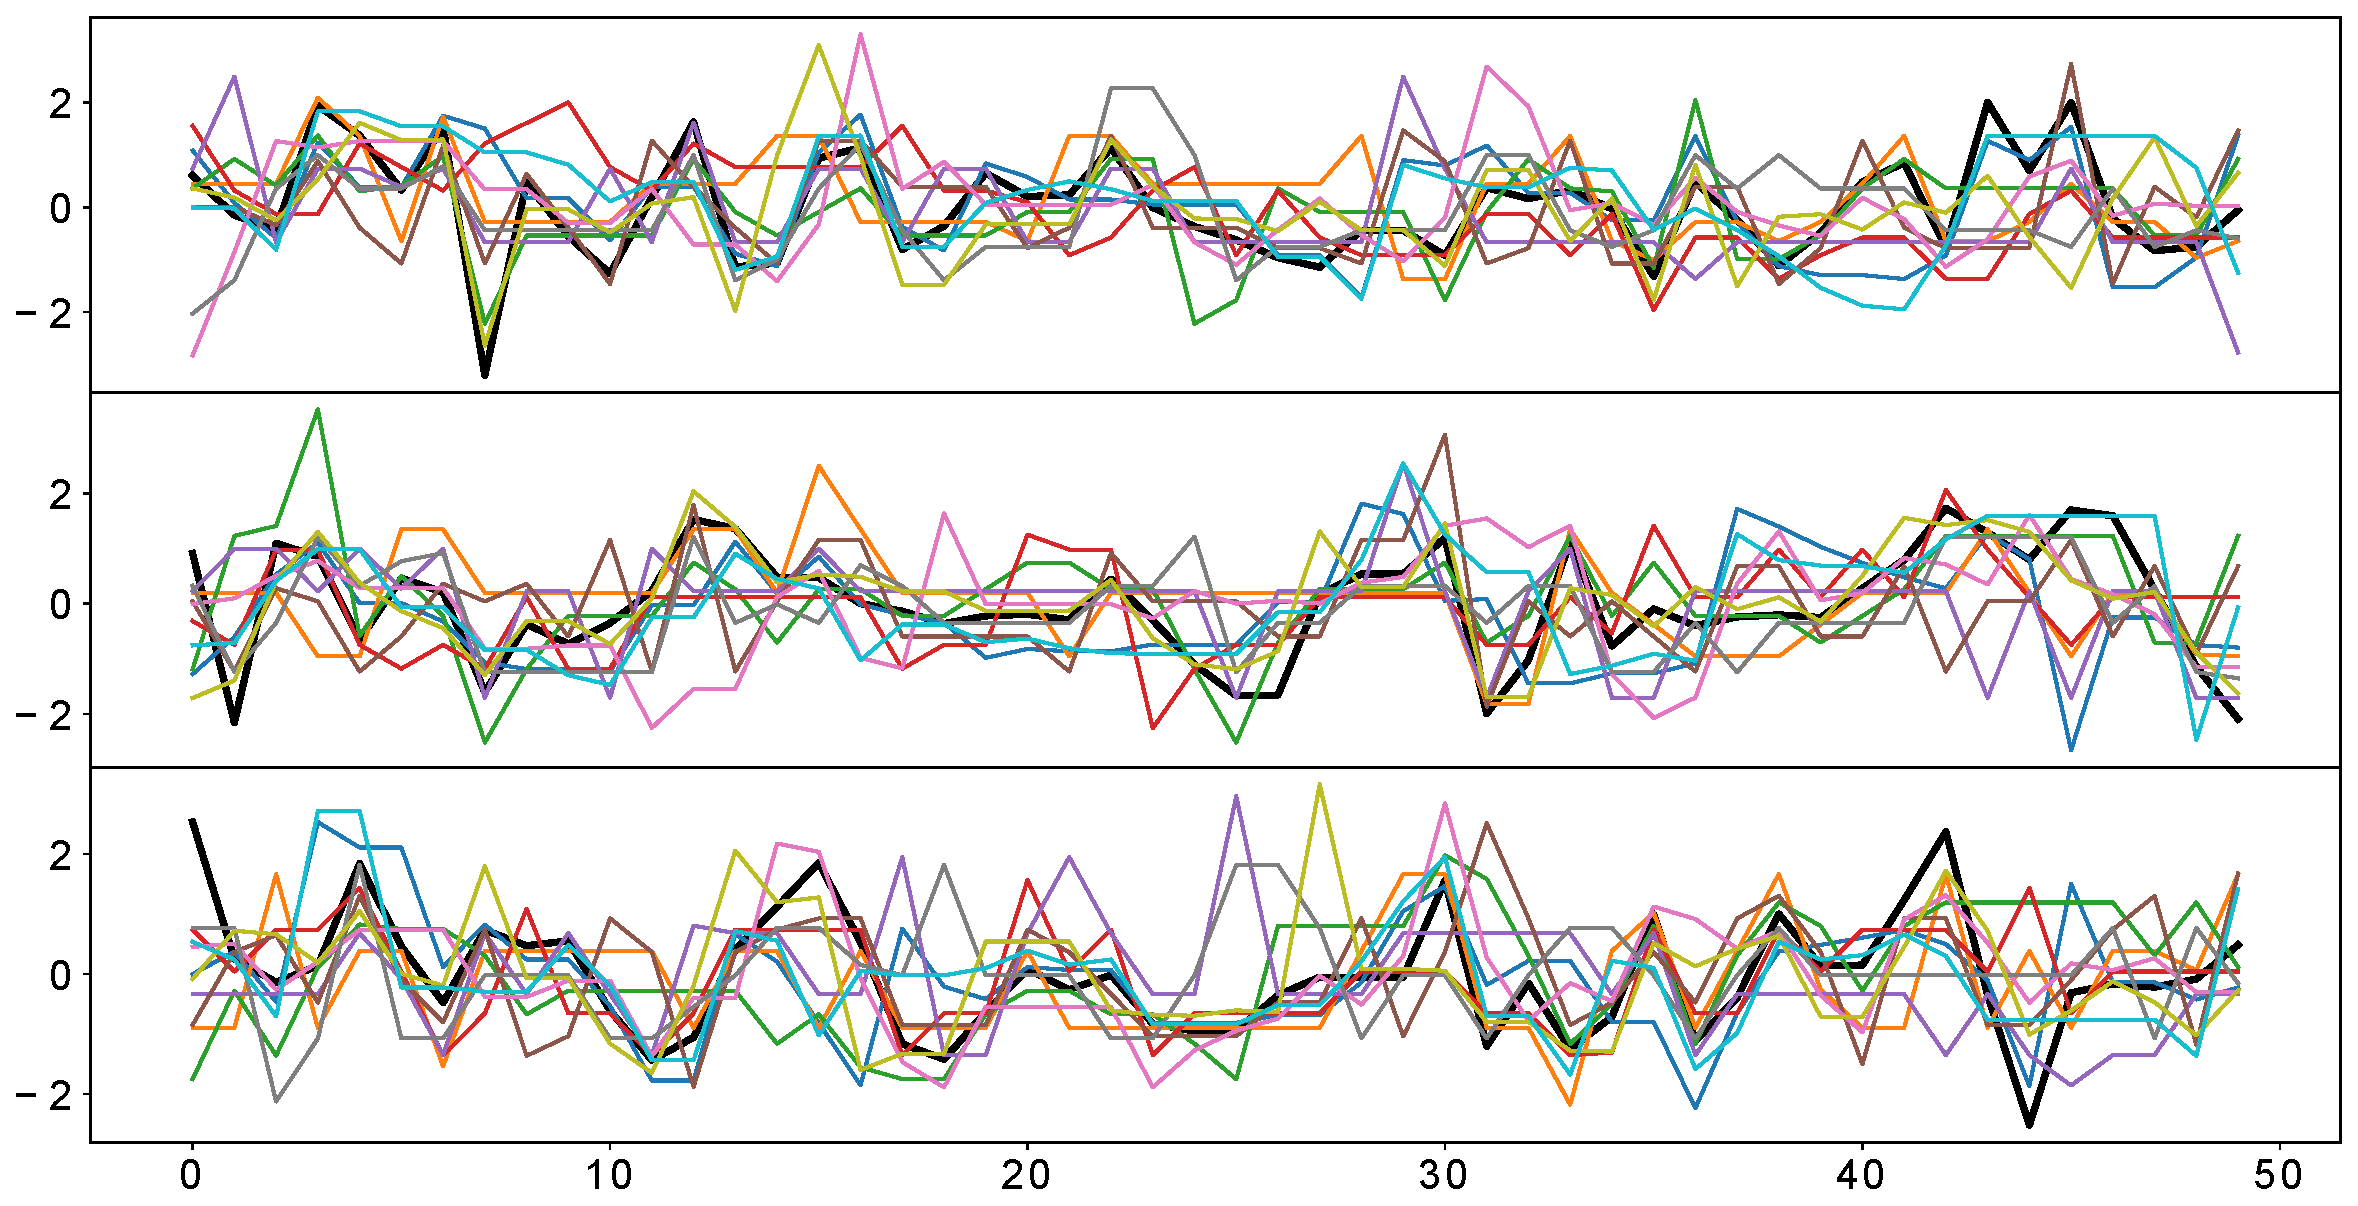
\includegraphics[width=\textwidth]{images/img2.eps}
        \caption{Кластеризация с $L_1$} \label{img1}
    \end{figure}
    \begin{figure}[h!]
        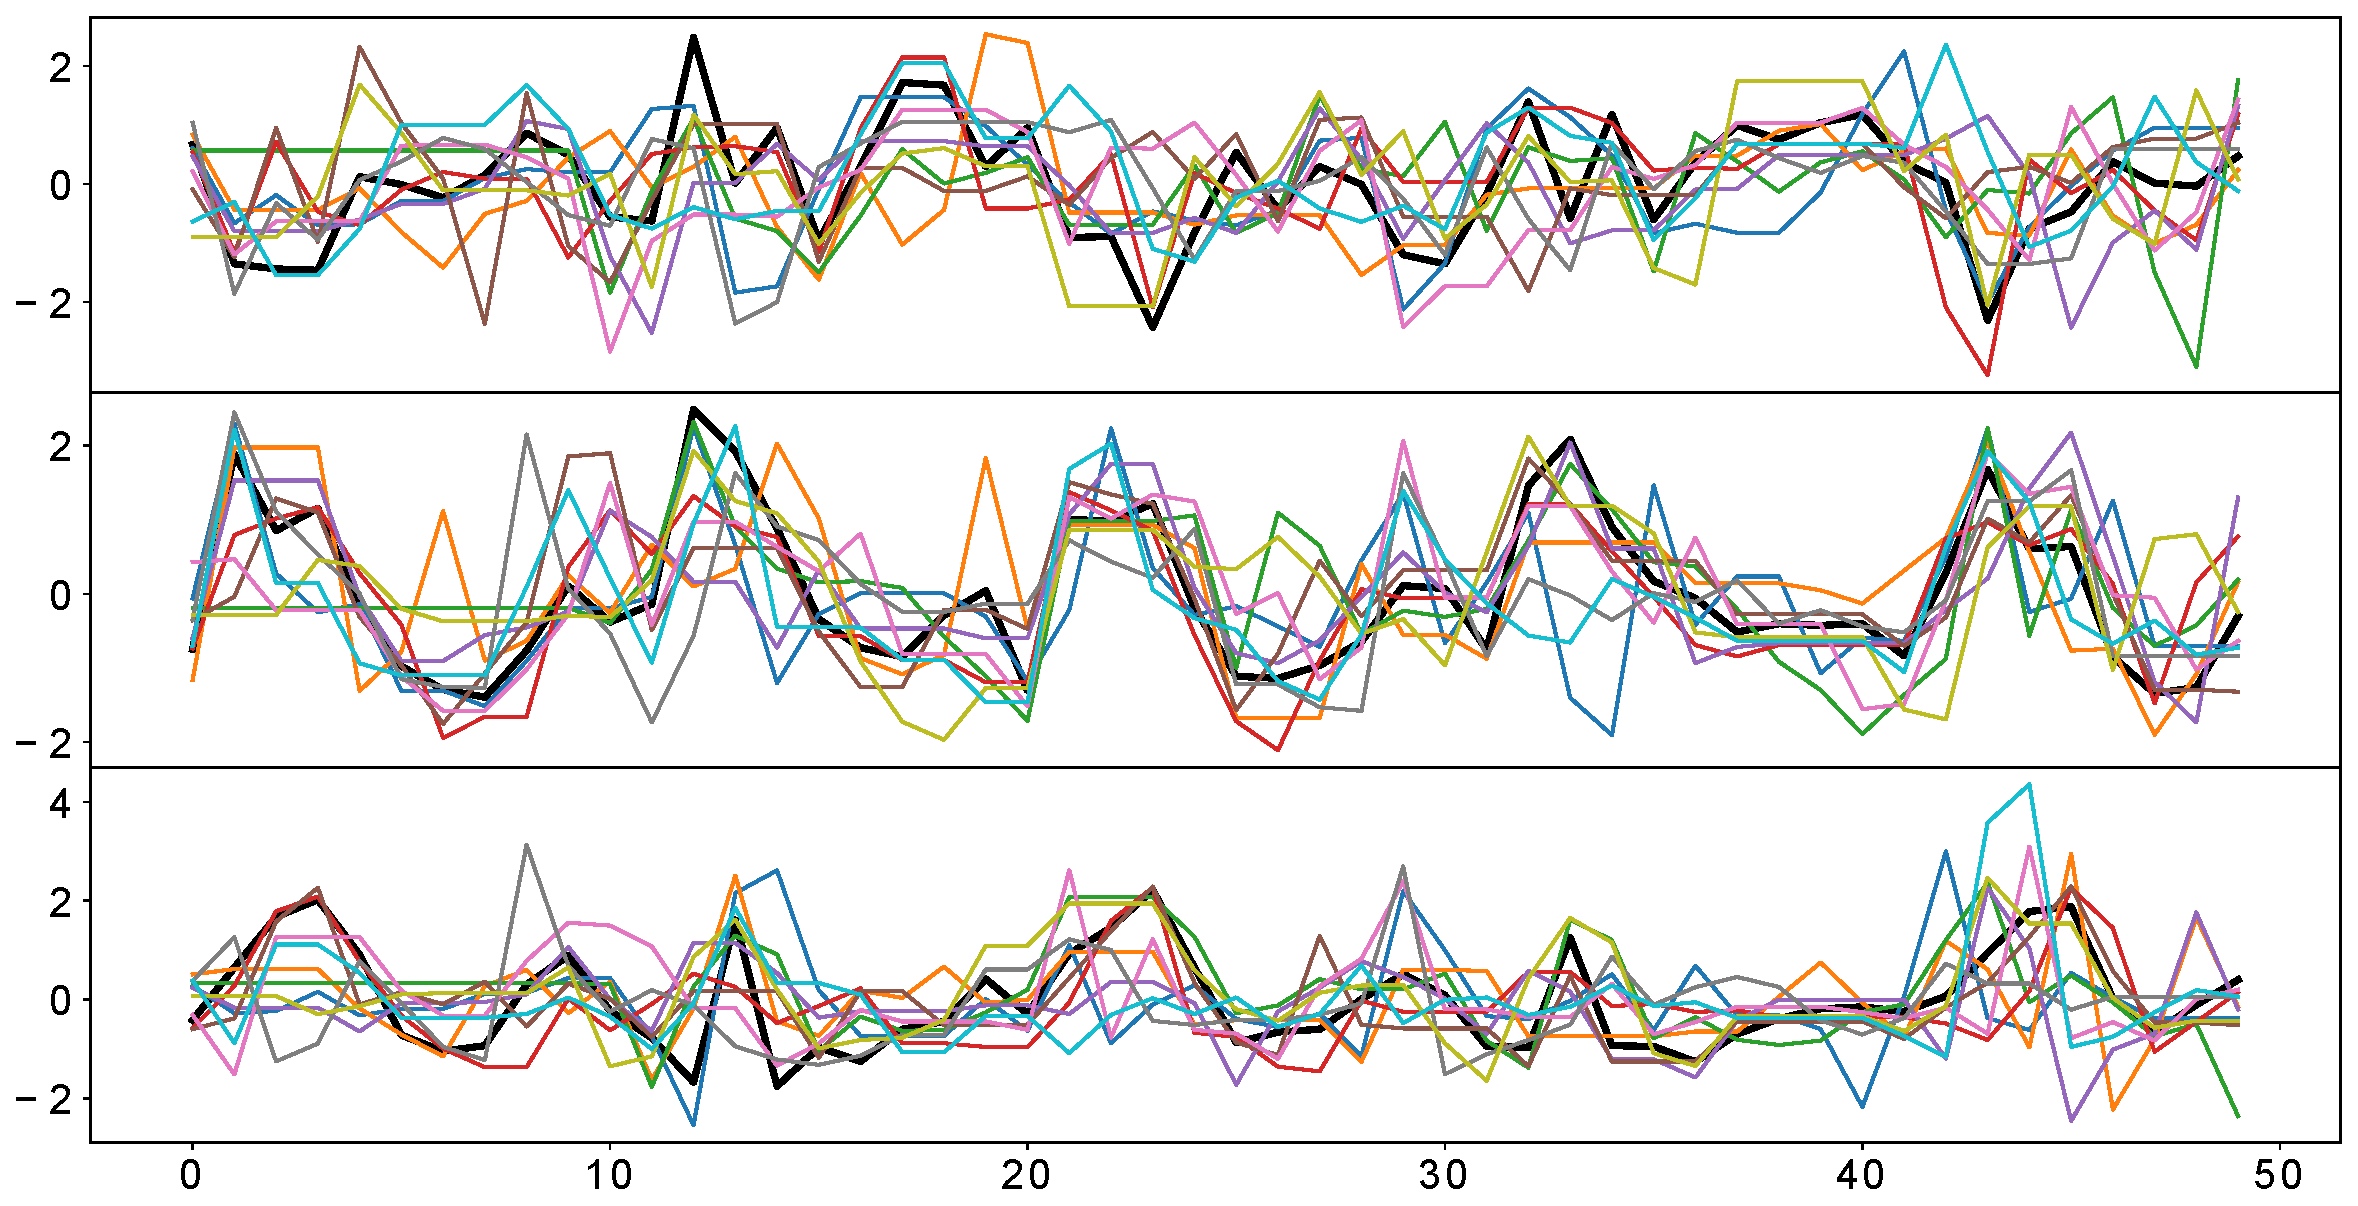
\includegraphics[width=\textwidth]{images/img3.eps}
        \caption{Кластеризация с $L_2$} \label{img2}
    \end{figure}                
    % \section{Заключение}
    
    

    \bibliography{literature} 
    \bibliographystyle{unsrt}
    
    % Решение Программного Комитета:
    %\ACCEPTNOTE
    %\AMENDNOTE
    %\REJECTNOTE
\end{document}
    

    
